\documentclass[a4paper,10pt]{article}
\usepackage[utf8]{inputenc}
\usepackage{graphicx}
\usepackage{fullpage}

\title{Example Title}
\author{Can Erdogan}

\begin{document}

\maketitle

\section{We have three types of section names - this is biggest}


\subsection{One smaller}
\subsubsection{Smallest}

\section{Section numbers are automatically generated}

\begin{figure}[!ht] 
  \centering
  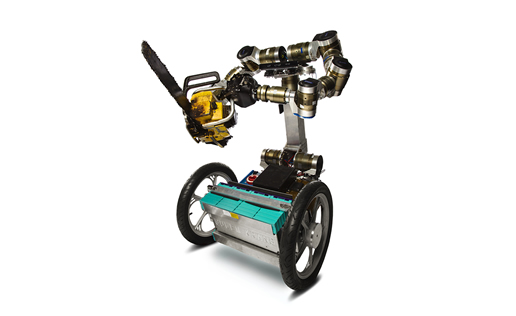
\includegraphics[width=1.0\columnwidth]{ex3.jpg}
  \caption{Play with the width variable of this image}
\end{figure}

That's it really. You usually write here. If you want a new paragraph, you need to make a newline
in the .tex

file just like this. Every paragraph is indented by default. If you want to include math, use
the \$ symbol at each end of your equation just like this: $x + y = 0.0$. There is tons of examples
online that you can refer to if you have any specific questions but for now this should suffice. 

\end{document}
